\documentclass[../../../../main.tex]{subfiles}
\begin{document}

\begin{flushright}
\footnotesize\textit{【自動文字起こし・要確認】}
\end{flushright}

[解] $C: x^2 + (y-1)^2 = 1$, $l: y = a(x+1)$

(1) Pから $l$ に下ろした垂足を H とする
\[ PH = \frac{|a-1|}{\sqrt{a^2+1}} \]
だから、
\[ HQ = \sqrt{1 - PH^2} = \sqrt{1 - \frac{(a-1)^2}{a^2+1}} = \sqrt{\frac{2a}{a^2+1}} \]
より
\[ \triangle PQR = \frac{1}{2} \cdot PH \cdot 2HQ = \frac{\sqrt{2a}|a-1|}{a^2+1} \]

(2) $0 < a < 1$ の時、
\[ \triangle PQR = S(a) = \frac{\sqrt{2a}(1-a)}{a^2+1} = \sqrt{\frac{2a(1-a)^2}{(a^2+1)^2}} \]
$\sqrt{\vphantom{x}}$ の中身を $f(a)$ とおく。
\begin{align*}
f'(a) &= 2 \frac{ (3a^2-4a+1)(a^2+1)^2 - a(1-a)^2 \cdot 2(a^2+1) \cdot 2a }{(a^2+1)^4} \\
&= \frac{2}{(a^2+1)^3} \left[ (3a-1)(a-1)(a^2+1) - 4a^2(1-a)^2 \right] \\
&= \frac{2(1-a)}{(a^2+1)^2} (a+1) (a^2-4a+1)
\end{align*}
から、下表をうる。

\begin{center}
\begin{tabular}{|c|c|c|c|c|c|}
\hline
$a$ & $0$ & $\cdots$ & $2-\sqrt{3}$ & $\cdots$ & $1$ \\
\hline
$f'$ & & $+$ & $0$ & $-$ & \\
\hline
$f$ & & $\nearrow$ & & $\searrow$ & \\
\hline
\end{tabular}
\end{center}
したがって、$S(a)$ も $a=2-\sqrt{3}$ で max をとる。

\begin{center}
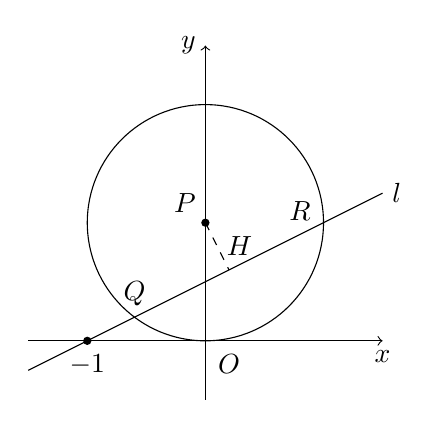
\begin{tikzpicture}[scale=1.5]
\draw[->] (-1.5, 0) -- (1.5, 0) node[below] {$x$};
\draw[->] (0, -0.5) -- (0, 2.5) node[left] {$y$};
\draw (0,1) circle (1);
\fill (0,1) circle (1pt) node[above left] {$P$};
\draw[domain=-1.5:1.5] plot (\x, {0.5*(\x+1)}) node[right] {$l$};
\fill (-1,0) circle (1pt);
\node at (-1, -0.2) {$-1$};
\node at (0.2, -0.2) {$O$};
\node at (-0.6, 0.4) {$Q$};
\node at (0.8, 1.1) {$R$};
\draw[dashed] (0,1) -- (0.2, 0.6) node[midway, right] {$H$};
\end{tikzpicture}
\end{center}

\end{document}
